\section{Результаты}
\subsection{Гистограмма и график плотности распределения}
\begin{figure}[H]
	\center{\includegraphics[width=1\linewidth]{task1\_images/Norm}}
	\caption{ Нормальное распределение.}
	\label{ris:1}
\end{figure}
\begin{figure}[H]
	\center{\includegraphics[width=1\linewidth]{task1\_images/Cauchy}}
	\caption{ Распределение Коши.}
	\label{ris:2}
\end{figure}
\begin{figure}[H]
	\center{\includegraphics[width=1\linewidth]{task1\_images/Laplace}}
	\caption{ Распределение Лапласа.}
	\label{ris:3}
\end{figure}
\begin{figure}[H]
	\center{\includegraphics[width=1\linewidth]{task1\_images/Poisson}}
	\caption{ Распределение Пуассона.}
	\label{ris:4}
\end{figure}
\begin{figure}[H]
	\center{\includegraphics[width=1\linewidth]{task1\_images/Uniform}}
	\caption{ Равномерное распределение.}
	\label{ris:5}
\end{figure}

\subsection{Характеристики положения и рассеяния}
\begin{table}[H]
	\begin{center}
		\begin{tabular}{|c|c|c|c|c|c|}
\hline
 & $\bar{x} \, (\ref{8})$ & $med \, x \, (\ref{9})$ & $z_R \, (\ref{10})$ & $z_Q \, (\ref{12})$ & $z_{tr} \, (\ref{13})$ \\
\hline
n =10 &  &  &  &  & \\
\hline
$E(z) \, (\ref{1})$ & -0.0037 & 0.0007 & -0.0069 & 0.3047 & 0.1071\\
\hline
$D(z) \, (\ref{2})$ & 0.0905 & 0.1237 & 0.1781 & 0.1149 & 0.0736\\
\hline
n =100 &  &  &  &  & \\
\hline
$E(z) \, (\ref{1})$ & -0.003 & -0.0063 & 0.0008 & 0.012 & 0.0091\\
\hline
$D(z) \, (\ref{2})$ & 0.0099 & 0.0154 & 0.0935 & 0.0128 & 0.0117\\
\hline
n =1000 &  &  &  &  & \\
\hline
$E(z) \, (\ref{1})$ & -0.0019 & -0.0013 & -0.0095 & 0.0002 & -0.0003\\
\hline
$D(z) \, (\ref{2})$ & 0.001 & 0.0016 & 0.0616 & 0.0013 & 0.0012\\
\hline
\end{tabular}
	\end{center}
	\caption{\label{tab:2} Нормальное распределение.}
\end{table}
\begin{table}[H]
	\begin{center}
		\begin{tabular}{|c|c|c|c|c|c|}
\hline
 & $\bar{x} \, (\ref{8})$ & $med \, x \, (\ref{9})$ & $z_R \, (\ref{10})$ & $z_Q \, (\ref{12})$ & $z_{tr} \, (\ref{13})$ \\
\hline
n =10 &  &  &  &  & \\
\hline
$E(z) \, (\ref{1})$ & 2.4504 & 0.0079 & 12.1986 & 1.2413 & 0.227\\
\hline
$D(z) \, (\ref{2})$ & 2303.6085 & 0.3383 & 57294.2839 & 5.7869 & 0.3439\\
\hline
n =100 &  &  &  &  & \\
\hline
$E(z) \, (\ref{1})$ & 0.7344 & 0.0045 & 33.2972 & 0.0471 & 0.0254\\
\hline
$D(z) \, (\ref{2})$ & 26405.1041 & 0.0251 & 65911815.5151 & 0.0513 & 0.0255\\
\hline
n =1000 &  &  &  &  & \\
\hline
$E(z) \, (\ref{1})$ & -38.6377 & -0.0005 & -19307.6697 & 0.0012 & 0.0008\\
\hline
$D(z) \, (\ref{2})$ & 1503091.5028 & 0.0025 & 375725093866.003 & 0.0051 & 0.0027\\
\hline
\end{tabular}
	\end{center}
	\caption{\label{tab:3} Распределение Коши.}
\end{table}
\begin{table}[H]
	\begin{center}
		\begin{tabular}{|c|c|c|c|c|c|}
\hline
 & $\bar{x} \, (\ref{8})$ & $med \, x \, (\ref{9})$ & $z_R \, (\ref{10})$ & $z_Q \, (\ref{12})$ & $z_{tr} \, (\ref{13})$ \\
\hline
n =10 &  &  &  &  & \\
\hline
$E(z) \, (\ref{1})$ & -0.0058 & -0.0073 & -0.0147 & 0.2931 & 0.0814\\
\hline
$D(z) \, (\ref{2})$ & 0.1066 & 0.0785 & 0.4171 & 0.1286 & 0.0543\\
\hline
n =100 &  &  &  &  & \\
\hline
$E(z) \, (\ref{1})$ & 0.0017 & 0.0023 & -0.0288 & 0.0174 & 0.0119\\
\hline
$D(z) \, (\ref{2})$ & 0.0103 & 0.0055 & 0.4444 & 0.0099 & 0.006\\
\hline
n =1000 &  &  &  &  & \\
\hline
$E(z) \, (\ref{1})$ & 0.0003 & 0.0 & 0.0448 & 0.001 & 0.001\\
\hline
$D(z) \, (\ref{2})$ & 0.001 & 0.0005 & 0.3915 & 0.001 & 0.0006\\
\hline
\end{tabular}
	\end{center}
	\caption{\label{tab:4} Распределение Лапласа.}
\end{table}
\begin{table}[H]
	\begin{center}
		\begin{tabular}{|c|c|c|c|c|c|}
\hline
 & $\bar{x} \, (\ref{8})$ & $med \, x \, (\ref{9})$ & $z_R \, (\ref{10})$ & $z_Q \, (\ref{12})$ & $z_{tr} \, (\ref{13})$ \\
\hline
n =10 &  &  &  &  & \\
\hline
$E(z) \, (\ref{1})$ & 9.9466 & 9.848 & 10.2235 & 10.869 & 8.5495\\
\hline
$D(z) \, (\ref{2})$ & 0.9182 & 1.3344 & 1.8508 & 1.2703 & 0.7974\\
\hline
n =100 &  &  &  &  & \\
\hline
$E(z) \, (\ref{1})$ & 9.9958 & 9.849 & 10.884 & 9.971 & 9.7027\\
\hline
$D(z) \, (\ref{2})$ & 0.0959 & 0.1917 & 0.94 & 0.1482 & 0.1095\\
\hline
n =1000 &  &  &  &  & \\
\hline
$E(z) \, (\ref{1})$ & 10.0037 & 9.998 & 11.669 & 9.9915 & 9.8468\\
\hline
$D(z) \, (\ref{2})$ & 0.0102 & 0.0015 & 0.6549 & 0.0042 & 0.0114\\
\hline
\end{tabular}
	\end{center}
	\caption{\label{tab:5} Распределение Пуассона.}
\end{table}
\begin{table}[H]
	\begin{center}
		\begin{tabular}{|c|c|c|c|c|c|}
\hline
 & $\bar{x} \, (\ref{8})$ & $med \, x \, (\ref{9})$ & $z_R \, (\ref{10})$ & $z_Q \, (\ref{12})$ & $z_{tr} \, (\ref{13})$ \\
\hline
n =10 &  &  &  &  & \\
\hline
$E(z) \, (\ref{1})$ & -0.0235 & -0.03 & -0.0147 & 0.2981 & 0.1061\\
\hline
$D(z) \, (\ref{2})$ & 0.0993 & 0.2299 & 0.0436 & 0.1234 & 0.1244\\
\hline
n =100 &  &  &  &  & \\
\hline
$E(z) \, (\ref{1})$ & 0.0065 & 0.0109 & 0.0001 & 0.0254 & 0.0267\\
\hline
$D(z) \, (\ref{2})$ & 0.0106 & 0.0304 & 0.0005 & 0.0158 & 0.0202\\
\hline
n =1000 &  &  &  &  & \\
\hline
$E(z) \, (\ref{1})$ & 0.0002 & 0.0003 & 0.0 & 0.002 & 0.0022\\
\hline
$D(z) \, (\ref{2})$ & 0.001 & 0.0028 & 0.0 & 0.0015 & 0.0019\\
\hline
\end{tabular}
	\end{center}
	\caption{\label{tab:6} Равномерное распределение.}
\end{table}

\subsection{Боксплот Тьюки}
\begin{figure}[H]
	\center{\includegraphics[width=0.65\linewidth]{task3\_data/Norm}}
	\caption{ Нормальное распределение.}
	\label{ris:6}
\end{figure}
\begin{figure}[H]
	\center{\includegraphics[width=0.65\linewidth]{task3\_data/Cauchy}}
	\caption{ Распределение Коши.}
	\label{ris:7}
\end{figure}
\begin{figure}[H]
	\center{\includegraphics[width=0.65\linewidth]{task3\_data/Laplace}}
	\caption{ Распределение Лапласа.}
	\label{ris:8}
\end{figure}
\begin{figure}[H]
	\center{\includegraphics[width=0.65\linewidth]{task3\_data/Poisson}}
	\caption{ Распределение Пуассона.}
	\label{ris:9}
\end{figure}
\begin{figure}[H]
	\center{\includegraphics[width=0.65\linewidth]{task3\_data/Uniform}}
	\caption{ Равномерное распределение.}
	\label{ris:10}
\end{figure}

\subsection{Доля выбросов}
\begin{table}[H]
	\begin{center}
		\begin{tabular}{|c|c|}
\hline
Sample & Share of emissions \\
\hline
Norm n = $20$ & $0.023$\\
\hline
Norm n = $100$ & $0.01$\\
\hline
Cauchy n = $20$ & $0.151$\\
\hline
Cauchy n = $100$ & $0.156$\\
\hline
Laplace n = $20$ & $0.075$\\
\hline
Laplace n = $100$ & $0.065$\\
\hline
Poisson n = $20$ & $0.022$\\
\hline
Poisson n = $100$ & $0.011$\\
\hline
Uniform n = $20$ & $0$\\
\hline
Uniform n = $100$ & $0$\\
\hline
\end{tabular}
	\end{center}
	\caption{\label{tab:7} Экспериментальная доля выбросов.}
\end{table}

\subsection{Теоретическая вероятность выбросов}
\begin{table}[H]
	\begin{center}
		\begin{tabular}{|c|c|}
			\hline
			Распределение & $P_B^T \,(\ref{17}),(\ref{18})$ \\
			\hline
			Нормальное распределение & 0.007\\
			\hline
			Распределение Коши  & 0.156\\
			\hline
			Распределение Лапласа & 0.063\\
			\hline
			Распределение Пуассона & 0.008\\
			\hline
			Равномерное распределение & 0\\
			\hline
		\end{tabular}
	\end{center}
	\caption{\label{tab:8} Теоретическая вероятность выбросов.}
\end{table}

\subsection{Эмпирическая функция распределения}
\begin{figure}[H]
	\center{\includegraphics[width=1\linewidth]{task4\_data/Norm\_emperic\_f}}
	\caption{ Нормальное распределение.}
	\label{ris:11}
\end{figure}
\begin{figure}[H]
	\center{\includegraphics[width=1\linewidth]{task4\_data/Cauchy\_emperic\_f}}
	\caption{ Распределение Коши.}
	\label{ris:12}
\end{figure}
\begin{figure}[H]
	\center{\includegraphics[width=1\linewidth]{task4\_data/Laplace\_emperic\_f}}
	\caption{ Распределение Лапласа.}
	\label{ris:13}
\end{figure}
\begin{figure}[H]
	\center{\includegraphics[width=1\linewidth]{task4\_data/Poisson\_emperic\_f}}
	\caption{ Распределение Пуассона.}
	\label{ris:14}
\end{figure}
\begin{figure}[H]
	\center{\includegraphics[width=1\linewidth]{task4\_data/Uniform\_emperic\_f}}
	\caption{ Равномерное распределение.}
	\label{ris:15}
\end{figure}

\subsection{Ядерные оценки плотности распределения}
\begin{figure}[H]
	\center{\includegraphics[width=1\linewidth]{task4\_data/Norm\_kernel\_n20}}
	\caption{ Нормальное распределение n = 20.}
	\label{ris:16}
\end{figure}
\begin{figure}[H]
	\center{\includegraphics[width=1\linewidth]{task4\_data/Norm\_kernel\_n60}}
	\caption{ Нормальное распределение n = 60.}
	\label{ris:17}
\end{figure}
\begin{figure}[H]
	\center{\includegraphics[width=1\linewidth]{task4\_data/Norm\_kernel\_n100}}
	\caption{ Нормальное распределение n = 100.}
	\label{ris:18}
\end{figure}
\begin{figure}[H]
	\center{\includegraphics[width=1\linewidth]{task4\_data/Cauchy\_kernel\_n20}}
	\caption{ Распределение Коши n = 20.}
	\label{ris:19}
\end{figure}
\begin{figure}[H]
	\center{\includegraphics[width=1\linewidth]{task4\_data/Cauchy\_kernel\_n60}}
	\caption{ Распределение Коши n = 60.}
	\label{ris:20}
\end{figure}
\begin{figure}[H]
	\center{\includegraphics[width=1\linewidth]{task4\_data/Cauchy\_kernel\_n100}}
	\caption{ Распределение Коши n = 100.}
	\label{ris:21}
\end{figure}
\begin{figure}[H]
	\center{\includegraphics[width=1\linewidth]{task4\_data/Laplace\_kernel\_n20}}
	\caption{ Распределение Лапласа n = 20.}
	\label{ris:22}
\end{figure}
\begin{figure}[H]
	\center{\includegraphics[width=1\linewidth]{task4\_data/Laplace\_kernel\_n60}}
	\caption{ Распределение Лапласа n = 60.}
	\label{ris:23}
\end{figure}
\begin{figure}[H]
	\center{\includegraphics[width=1\linewidth]{task4\_data/Laplace\_kernel\_n100}}
	\caption{ Распределение Лапласа n = 100.}
	\label{ris:24}
\end{figure}
\begin{figure}[H]
	\center{\includegraphics[width=1\linewidth]{task4\_data/Poisson\_kernel\_n20}}
	\caption{ Распределение Пуассона n = 20.}
	\label{ris:25}
\end{figure}
\begin{figure}[H]
	\center{\includegraphics[width=1\linewidth]{task4\_data/Poisson\_kernel\_n60}}
	\caption{ Распределение Пуассона n = 60.}
	\label{ris:26}
\end{figure}
\begin{figure}[H]
	\center{\includegraphics[width=1\linewidth]{task4\_data/Poisson\_kernel\_n100}}
	\caption{ Распределение Пуассона n = 100.}
	\label{ris:27}
\end{figure}
\begin{figure}[H]
	\center{\includegraphics[width=1\linewidth]{task4\_data/Uniform\_kernel\_n20}}
	\caption{ Равномерное распределение n = 20.}
	\label{ris:28}
\end{figure}
\begin{figure}[H]
	\center{\includegraphics[width=1\linewidth]{task4\_data/Uniform\_kernel\_n60}}
	\caption{ Равномерное распределение n = 60.}
	\label{ris:29}
\end{figure}
\begin{figure}[H]
	\center{\includegraphics[width=1\linewidth]{task4\_data/Uniform\_kernel\_n100}}
	\caption{ Равномерное распределение n = 100.}
	\label{ris:30}
\end{figure}